\chapter{Electro-kinetics -- 2D -- Electro-osmotic flow and advected species}

\modinfo{Directory}{Electrokinetics}
\modinfo{Solvers}{\Idx{StatElecSolve}, \Idx{FlowSolve},  \Idx{AdvectionDiffusion}, \Idx{Electrokinetics}}
\modinfo{Tools}{\Idx{ElmerGUI}}
\modinfo{Dimensions}{2D, Transient}
\modinfo{Author}{Original author not known}

\subsection*{Case definition}

This tutorial is an example of setting up a simulation for (microfluidic) electro-osmotic flow advecting a passive scalar quantity. Diffusion of the species is also included. The geometry of the system is a simple 2D microchannel with T crossing. The flow is induced by the applied electric field and the electric double layer at the channel walls. The analyte (species) is inserted into the system from the left hand side inlet.

More details on the electro-kinetic capabilities of Elmer are found on the Models Manual, chapter ``Electrokinetics'', authored by T. Zwinger.

This is an old case of analyte transport with \Idx{Helmholtz-Smoluchowski} Boundary Conditions.  Not perhaps particularly accurate as the advection-diffusion equation suffers  from high numerical diffusion. Particularly for purely advective transport  the particle based methods might be more favourable. 

The geometry for this tutorial looks like as shown in figure \ref{fg:geometry}.

\begin{figure}[H]
\centering
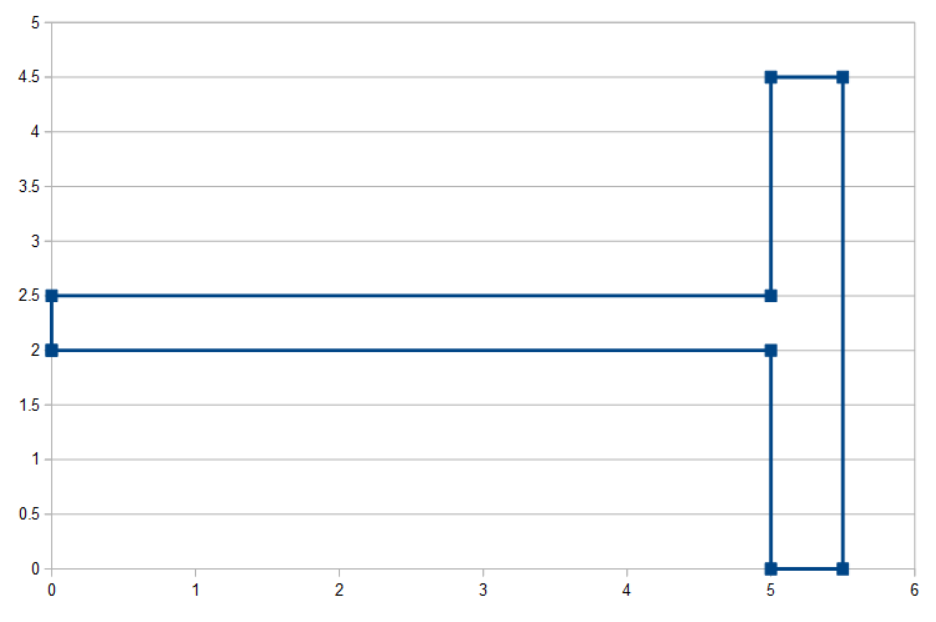
\includegraphics[width=0.7\textwidth]{geometry.png}
\caption{Geometry}\label{fg:geometry}
\end{figure}  

\subsection*{ElmerGUI Equation Menu}

The GUI definitions of Advection Diffusion solver utilized in this tutorial are located in the \texttt{edf-extra} folder and thus need to be manually activated in the ElmerGUI.\\

Note that the extra definition needs to be loaded first, before any other steps in building any tutorial.  Once the extra definition has been loaded, and the ElmerGUI project has been saved, then the reference to the extra definition will be stored in the project, and you won't have to load the extra definition again.

\begin{verbatim}
File
  Definitions
    Append -> advection-diffusion.xml
  Close
\end{verbatim}

\noindent The \texttt{\Idx{advection-diffusion.xml}} definition file is, by default, located in Linux in:

\texttt{\$ELMER\_HOME/share/ElmerGUI/edf-extra}

\noindent and in Windows, located in:

\texttt{C:/Program Files/Elmer 9.0-Release/share/ElmerGUI/edf-extra}\\

We will also be using the \Idx{Stat Elec Solver}, and the \Idx{Flow Solver}  which are two of the default, pre-loaded GUI definitions, so they do not need to be manually activated.  For reference, the  \texttt{\Idx{electrostatics.xml}}  and the  \texttt{\Idx{navier-stokes.xml}} definition files are, by default, located in Linux in:

\texttt{\$ELMER\_HOME/share/ElmerGUI/edf}

\noindent and in Windows, located in:

\texttt{C:/Program Files/Elmer 9.0-Release/share/ElmerGUI/edf}\\

The \Idx{Electrokinetics solver} is used for a boundary condition and will be called when needed.  The Electrokinetics solver is located in the \texttt{\$ELMER\_HOME/bin} folder.

\subsection*{Solution procedure}

The mesh is given in ElmerGrid format in file \texttt{Tcross.grd}, load this file.

\ttbegin
File 
  Open -> Tcross.grd
\ttend

You should obtain your mesh and may check \texttt{Model Summary...} that it consists of 1200 surface elements.  Your mesh should look like as shown in figure \ref{fg:mesh}

\begin{figure}[H]
\centering
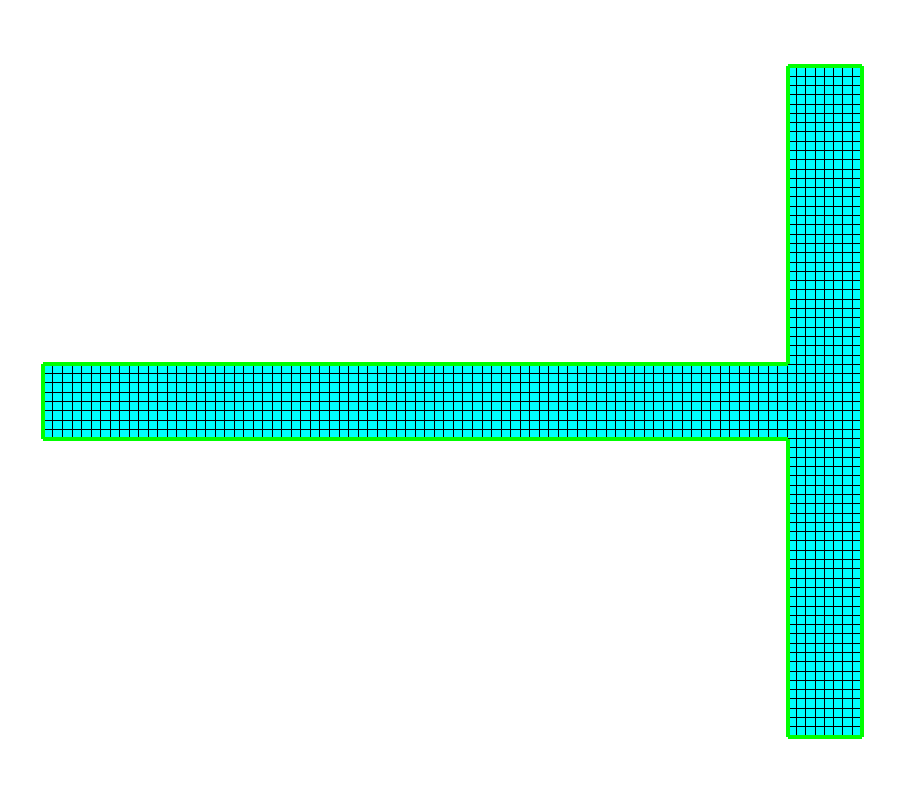
\includegraphics[width=0.7\textwidth]{mesh}
\caption{Mesh}\label{fg:mesh}
\end{figure}

After we have the mesh we start to go through the Model menu from the top to bottom.  In the Setup we choose things related to the whole simulation such as file names, time stepping, constants etc.  

The simulation is carried out in 2-dimensional Cartesian coordinates.  2nd order bdf time stepping method is selected with 120 steps and with step size of 1e-5 seconds.  Coordinate scaling reduces the size of the mesh and produces a T-shaped micro channel.


\ttbegin
Model
  Setup 
    Simulation Type = Transient
    Steady state max. iter = 20
    Timestepping method = BDF
    BDF order = 2
    Time Step Intervals = 120
    Timestep sized = 1e-5
    Output intervals = 2
    Coordinate Scaling = 1e-5 1e-5 1e-5
  Apply
\ttend

In the equation section we choose the relevant equations and parameters related to their solution.  In this case we'll have one set of equations (named ``Equation'') which consists of the Stat Electric equation, the Navier-Stokes equation, and the Advection Diffusion equation.\\

All three solvers are active in this equation set. Further definitions include, first, that the convection of the species is switched on (besides diffusion). Then that for Navier-Stokes equations the convective term may be left out resulting in laminar Stokes flow, and finally that the electric field is computed by the electrostatics rather than given by the user. \\

Note that the entry under Electrostatics of ``Electric Field = Computed'' may not exist in early versions of the ElmerGUI menu definition in the electrostatics.xml file.  When the Solver is run, an error may be reported, such as ``electrokinetics helmholtz  smoluchowski: No external electric field defined for Equation 1''.  If this occurs, either update your version of Elmer, or generate the .sif file manually, then add this statement \texttt{Electric Field = Computed} in the Equation block, and run the solver manually.

When defining Equations and Materials it is possible to assign to the bodies immediately, or to use mouse selection to assign them later. In this case we have just one body and therefore its easier to assign the Equation and Material to it directly.  

The electrostatics equation is linear and thus no non-linear iterations are needed. The equation is solved using a fast direct method UMFPack.

The system may include non-linear iterations of each equation and steady state iterations to obtain convergence of the coupled system. It is often a good idea to keep the number of non-linear iterations in a coupled case low.  Here we select just  a maximum of 30 non-linear iterations for the Navier-Stokes equation.

The advection-diffusion equation does not affect either the electrostatic field or the flow, thus it may be solved only after a converged solution for the previous two equations is available. This is achieved with the \texttt{After timestep} definition below. The advected quantity is called Concentration.  The advection-diffusion solver uses bubble stabilization method to avoid numerical problems associated with convection type equations.\\

\ttbegin
Model
  Equation
   Name = Equation 1
    Apply to Bodies = 1
    Electrostatics
      Active = True, checked
      Electric Field = Computed
      Edit Solver Settings
      General
        Before timestep
      Solver specific options
        Calculate Electric Field = True
      Linear system
        Method
          Direct = Umfpack
        Preconditioning = ILU1
     Apply
     Navier-Stokes
       Active = True, checked
       Options
         Convect = unchecked, False
      Edit Solver Settings
       Linear system
         Preconditioning = ILU1
       Nonlinear system
         Max. iterations = 30
         Newton
           After iterations = 10
     Apply
     Advection Diffusion
        Active = True, checked
        Concentration Units = Absolute Mass
        Convection = Computed
      Edit Solver Settings
       General
         After timestep = True
         Stabilize = False
         Bubbles = True
       Linear system
         Preconditioning = ILU2
       Nonlinear system
         Max. iterations = 1
     Apply
    Add
    OK
\ttend        
The Material section includes all the material parameters. They are divided into generic parameters which are direct properties of the material without making any assumptions on the physical model, such as the mass. Other properties assume a physical law, such as conductivities and viscosity. \\

We use a material similar to water for this example.

\ttbegin
Model
  Material
    Name = Material 1
    Apply to Bodies = 1 
      General
        Density = 1e3
      Electrostatics
        Relative Permittivity = 1.0
      Navier-Stokes
        Viscosity = 1e-03
      Advection Diffusion
        Concentration Diffusivity = 1e-10
    Add
    OK
\ttend

A Body Force represents the right-hand-side of a equation. It is generally not a required field for a body.   No body force is included in this example.

Initial conditions should be given to transient cases, and probably are not needed for steady state solutions. No initial condition is used for this example.

Only one boundary condition may be applied to each boundary and therefore all the different physical BCs for a boundary should be grouped together. 

Finally the boundary conditions are defined. The first BC is given for the channel walls. Here, tangential velocity (velocity components 1 and 2) is computed by the Helmholtz-\Idx{Smoluchowski} slip velocity condition, which means that the velocity is computed using the computed electric field and the \Idx{electro-osmotic mobility} as inputs. 

\ttbegin
Model
  BoundaryCondition
    Name = channel-walls
    General
      Free text input
        EO Mobility = Real 5e-08
    Navier-Stokes 
      Velocity 1 = Variable Pressure
         Real Procedure  "Electrokinetics" "helmholtz_smoluchowski1"
      Velocity 2 = Variable Pressure
         Real Procedure  "Electrokinetics" "helmholtz_smoluchowski2"
    Add
    OK
\ttend  

The next BC is the inlet condition. We give a potential of 100 Volts and define that there is no flow in $y$-direction. The analyte concentration at the inlet is defined as a function of time using table format. The concentration is 1.0 up until time instant $3\cdot 10^{-5}$, is zero after $4\cdot 10^{-5}$s and decreases linearly between these two time instants.

\ttbegin
Model
  BoundaryCondition
    Name = inlet-el-A
    Electrostatics
     Potential = 100
    Navier-Stokes 
      Velocity 2 = 0.0
    Advection Diffusion
      Dirichlet Conditions
        Concentration
            Variable Time
              Real
              0.0     1.0
              3.0e-5  1.0
              4.0e-5  0.0
              0.5     0.0
           End           
    Add
   OK 
\ttend   

The final two boundary conditions are for the outlets. Different potentials for these are defined as well as a condition for velocity component.

\ttbegin
Model
  BoundaryCondition
    Name = outlet-el-B
    Electrostatics
     Potential = 30
    Navier-Stokes 
      Velocity 1 = 0.0         
    Add
   OK 
\ttend   

\ttbegin
Model
  BoundaryCondition
    Name = outlet-el-C
    Electrostatics
     Potential = 0
    Navier-Stokes 
      Velocity 1 = 0.0         
    Add
   OK 
\ttend   

The conditions may also be assigned to boundaries in the Boundary condition menu, or by clicking on each boundary with the mouse. Here we use the latter approach as that spares us of the need to know the indexes of each boundary.

\ttbegin
Model
  Set boundary properties
    Choose Inlet -> set boundary condition inlet-el-A
    Choose Top Outlet -> set boundary condition outlet-el-B
    Choose Bottom Outlet -> set boundary condition outlet-el-C
    Choose Walls -> set boundary condition channel-walls
   OK 
\ttend

For the execution ElmerSolver needs the mesh files and the command file.  We have now basically defined all the information for ElmerGUI to write the command file. After writing it we may also visually inspect the command file.
\ttbegin
Sif 
  Generate
  Edit -> look how your command file came out  
\ttend

Before we can execute the solver we should save the files in a directory.  The ElmerGUI project includes all the files needed to restart the case.

\ttbegin
File 
  Save Project
\ttend

After we have successfully saved the files we may start the solver.

\ttbegin
Run
  Start solver
\ttend

A convergence view automatically pops up showing relative changes of each iteration.\\

When there are some results to view we may start the postprocessor also.

\ttbegin
Run
  Start ParaView
\ttend

\subsection*{Results}

Due to the number of the time steps the simulation may take around 15 seconds.\\

You may inspect the results with Paraview or with ElmerVTK.\\

In Figure \ref{fg:time} the obtained concentration distribution is presented. 

\begin{figure}[H]
\centering
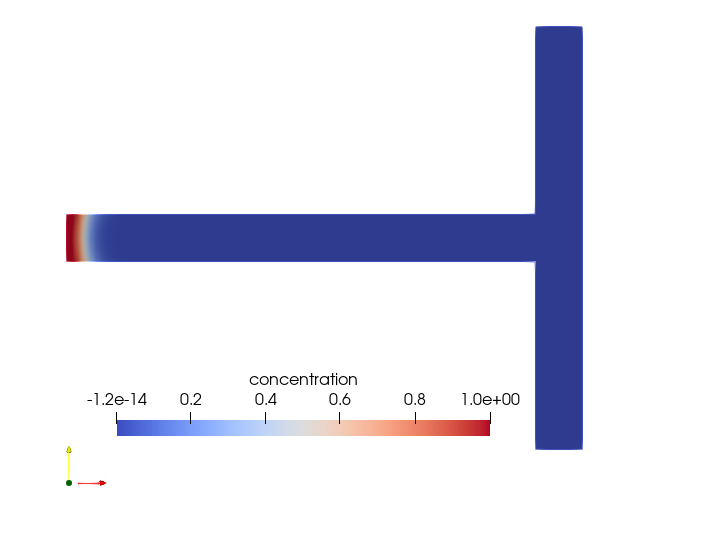
\includegraphics[width=0.48\textwidth]{time-0-ticks}
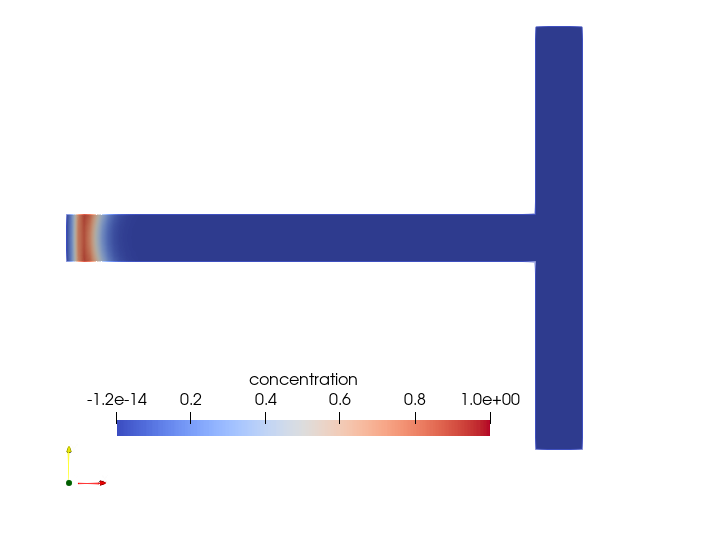
\includegraphics[width=0.48\textwidth]{time-2-ticks}
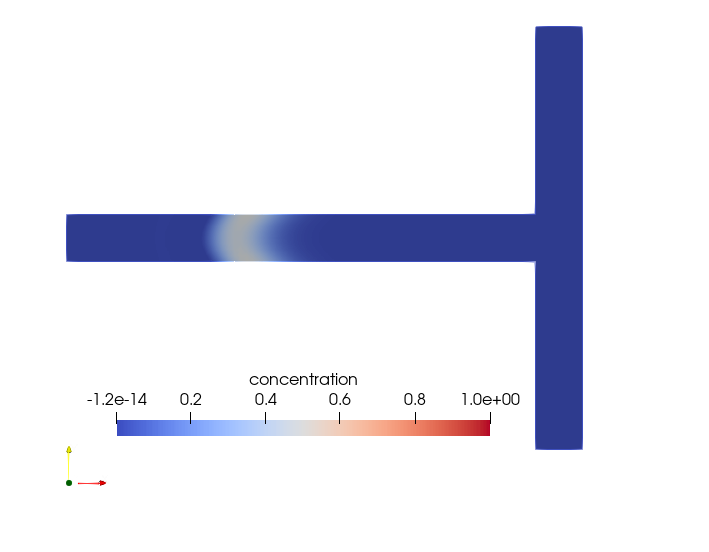
\includegraphics[width=0.48\textwidth]{time-15-ticks}
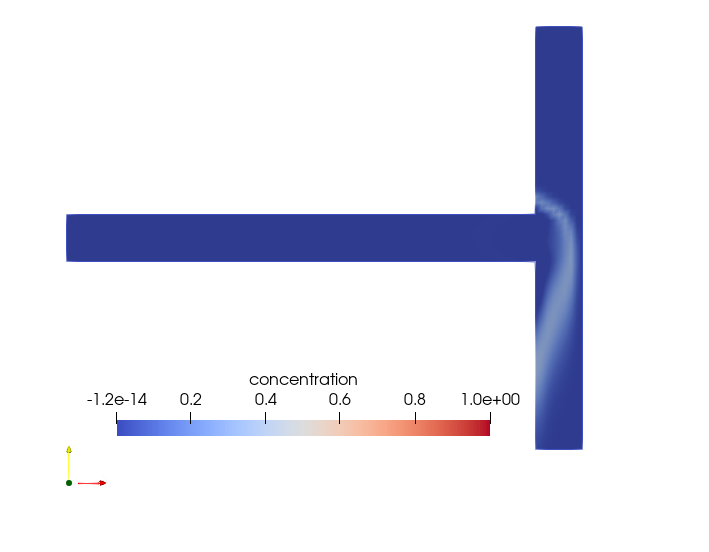
\includegraphics[width=0.48\textwidth]{time-45-ticks}
\caption{Concentration at time: 0, 2, 15, and 45 ticks}\label{fg:time}
\end{figure} 


\hfill
